\documentclass[12pt]{article}
\usepackage{times} 			% use Times New Roman font

\usepackage[margin=1in]{geometry}   % sets 1 inch margins on all sides
\usepackage[hidelinks]{hyperref}               % for URL formatting
\usepackage[pdftex]{graphicx}       % So includegraphics will work
\setlength{\parskip}{1em}           % skip 1em between paragraphs
\usepackage{indentfirst}            % indent the first line of each paragraph
\usepackage{datetime}
\usepackage[small, bf]{caption}
\usepackage{listings}               % for code listings
\usepackage{xcolor}                 % for styling code
\usepackage{multirow}
\usepackage{adjustbox}
\usepackage{caption}


%New colors defined below
\definecolor{backcolour}{RGB}{246, 246, 246}   % 0xF6, 0xF6, 0xF6
\definecolor{codegreen}{RGB}{16, 124, 2}       % 0x10, 0x7C, 0x02
\definecolor{codepurple}{RGB}{170, 0, 217}     % 0xAA, 0x00, 0xD9
\definecolor{codered}{RGB}{154, 0, 18}         % 0x9A, 0x00, 0x12

%Code listing style named "gcolabstyle" - matches Google Colab
\lstdefinestyle{gcolabstyle}{
  basicstyle=\ttfamily\small,
  backgroundcolor=\color{backcolour},   
  commentstyle=\itshape\color{codegreen},
  keywordstyle=\color{codepurple},
  stringstyle=\color{codered},
  numberstyle=\ttfamily\footnotesize\color{darkgray}, 
  breakatwhitespace=false,         
  breaklines=true,                 
  captionpos=b,                    
  keepspaces=true,                 
  numbers=left,                    
  numbersep=5pt,                  
  showspaces=false,                
  showstringspaces=false,
  showtabs=false,                  
  tabsize=2
}

\lstset{style=gcolabstyle}      %set gcolabstyle code listing

% to make long URIs break nicely
\makeatletter
\g@addto@macro{\UrlBreaks}{\UrlOrds}
\makeatother

% for fancy page headings
\usepackage{fancyhdr}
\setlength{\headheight}{13.6pt} % to remove fancyhdr warning
\pagestyle{fancy}
\fancyhf{}
\rhead{\small \thepage}
\lhead{\small HW\#8, Huang}  % EDIT THIS, REPLACE # with HW number
\chead{\small DATA 440, Fall 2022} 

%-------------------------------------------------------------------------
\begin{document}

% EDIT THE ITEMS HERE
\begin{centering}
{\large\textbf{Clustering}}\\ 
Sofia Huang\\
due 12/8/2022\\
\end{centering}

%-------------------------------------------------------------------------

% The * after \section just says to not number the sections
\section*{1. Find Popular Twitter Accounts}
\noindent \textbf{Generate a list of 100 popular accounts on Twitter. The accounts must be verified, have 10,000+ followers, and have 5000+ tweets. For example:
You may also generate this information manually by visiting individual account pages. You only need 100 popular accounts, so manual selection might be justified.
Because we're trying to cluster the accounts based on the text in their tweets, you should choose several sets of accounts that are similar (political, tech, sports, etc.) to see if they'll get clustered together later.
Save the list of accounts (screen\_names), one per line, in a text file named accounts.txt and upload to your GitHub repo.}

\noindent\textbf{A: How did you choose to collect the accounts?}

I chose to manually collect the accounts since it was only 100 and when I tried to collect them using twarc, the accounts were unfamiliar to me and I wanted to be able to easily see if the results of the clusters were as I expected which is hard to do when I do not know what the accounts are for. 

\noindent\textbf{B: What topics/categories do the accounts belong to? You don't need to specify a grouping for each account, but what general topics/categories will you expect to be revealed by the clustering? Provide a this list before generating your clusters}

I chose accounts across several categories including celebrities, news, sports, nature, travel, and food.

\section*{2. Create Account-Term Matrix}
\noindent \textbf{Before we can run the clustering code from the PCI book, we have to build an account-term matrix (like the blog-term matrix in the Module 12 slides). Consider the Twitter accounts equivalent to blogs, and all account tweets, the words of the blog.}

\noindent \textbf{A. Explain the general operation of generate\_tweet\_vector.py and how the tweets are converted to the account-term matrix.}

generate\_tweet\_vector.py parses each Twitter account and gets 100 tweets from their timeline. Then, it filters the words in the tweets, removing any URLs, other usernames, etc., and returns the account name and dictionary of word counts from that accounts' tweets. This process is repeated for every account and all of the data is stored in a dictionary (wordcounts).

Then, for each word, it counts the number of accounts it appears in and the total number of instances it appeared and stores these statistics in dictionaries (apcounts and sumcounts). 

Next, it iterates through the dictionary containing the number of counts a word appears in (apcounts) and find the fraction of how many times the word appears per all of the accounts. If it is between 0.1 and 0.5 it is added to a list.

Then, I used the dictionary containing the total count of times a word appeared over all accounts (sumcounts) to create a list (popularlist) of the 500 most frequent words over all of the accounts (more details on my code below). 

Finally, the tweet-term matrix, a .txt file, is created by writing out the most frequent words as the top row, then for each subsequent row, the account name is written, followed by the frequency of times each word in popularlist using the data stored in the wordcounts dictionary. 


\noindent \textbf{B: Explain in detail the code that you added to filter for the 500 most frequent non-stopword terms.}

First, I sorted the sum\_counts dictionary by the values in reverse order. This resulted in a list of tuples (key and value pair), ordered (descending) by the frequency of the words. I converted this list back into a dictionary and put the first 500 keys into a list, leaving me with the 500 most frequent non-stopword terms.

\begin{lstlisting}[language=bash, label=lst:copy]
sorted_sum_counts = dict(sorted(sumcounts.items(), key=lambda x:x[1], reverse=True))
popularlist = list(sorted_sum_counts.keys())[0:500]
\end{lstlisting}

\noindent \textbf{C: Do the 500 most frequent terms make sense based on the accounts that you chose?}

Yes, they do make sense. The most frequent words are pretty generic, ie. 'the', 'and', 'this', etc. But, words based on specific account categories appeared like 'season' and 'team' for sports or 'ocean' and 'earth' for nature accounts. 

\section*{3. Create Dendrogram}
\noindent \textbf{Create an ASCII dendrogram and a JPEG dendrogram that uses hierarchical clustering to cluster the most similar accounts (see Module 12, slides 21, 23). Include the JPEG in your report and upload the ASCII file to GitHub (it will be too unwieldy for inclusion in the report).}

\clearpage

\begin{figure}[h]
    \centering
    % trim and clip are used to crop the image, trim=left bottom right top
    % width sets max width, height will be scaled appropriately
    %\includegraphics[trim=0 20 10 50, clip, width=\textwidth]
    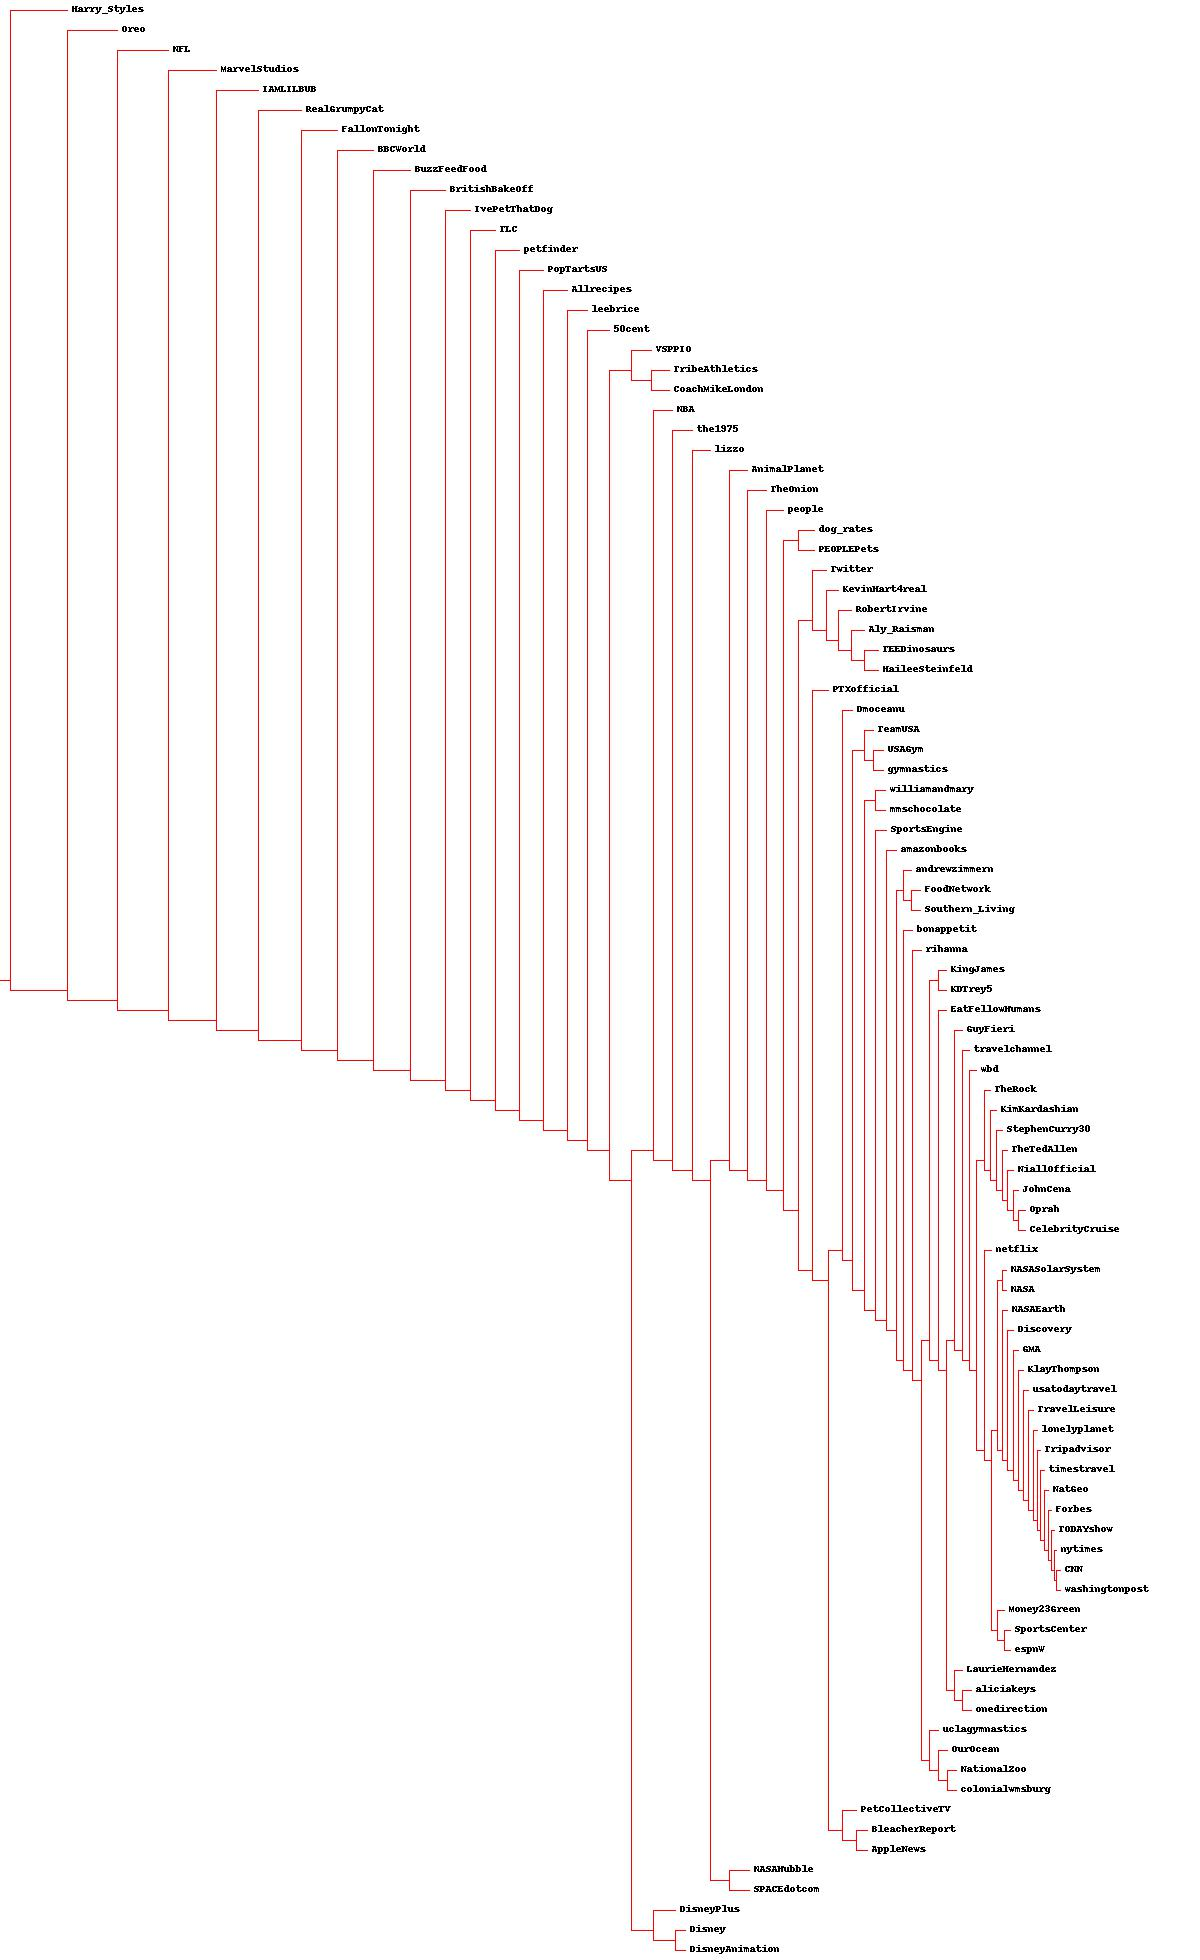
\includegraphics[width=300pt, scale=1]
    {accountclust.jpg}
    \caption{Twitter Account Dendrogram}
    \label{fig:dendrogram}
\end{figure}

\clearpage

\noindent \textbf{A: How well did the hierarchical clustering do in grouping similar accounts together? Were there any particularly odd groupings?}

The heirarchical clustering did pretty well in grouping similar accounts like @espn and @SportsCenter, and @onedirection and @aliciakeys, and many of the news accounts were grouped together. However, there were definitely a few odd groupings, such as @williamandmary and @mmschocolate.  

\section*{4. Cluster using k-Means}
\noindent \textbf{Cluster the accounts using k-Means, using k=5,10,20 (see Module 12, slide 34). For each value of k, create a file that lists the accounts in each cluster and upload to your GitHub repo.}

\noindent \textbf{A: Give a brief explanation of how the k-Means algorithm operates on this data. What features is the algorithm considering?}

First, k number of centroids are placed within the data. Then, using Pearson's distance, for each data point, find the centroid closest to it and assign the data point to that centroid's cluster. Once all of the data points have been assigned, move each centroid to the average point between all of its assigned data points. Repeat the process until the centroids do not move anymore and the data points are assigned to the correct centroid or cluster.

This algorithm is using the word counts from the tweet-term matrix to calculate the distances. 

\noindent \textbf{B: How many iterations were required for each value of k?}

For a value of 5 for k, 3 iterations were required (0-2).

For a value of 10 for k, 7 iterations were required (0-6).

For a value of 20 for k, 6 iterations were required (0-5).


\noindent \textbf{C: Which k value created the most reasonable clusters? For that grouping, characterize the accounts that were clustered into each group.}

A k value of 10 created the most reasonable clusters. Out of the 10 clusters created, 3 of them were empty. The first clusetr was comprised of mostly news and nature/travel related accounts. The second cluster had @PopTartsUS and @Oreo which are both big food brands. The third cluster was a little more varied and included William and Mary related accounts, as well as, movie studios (@Disney and @MarvelStudios etc.) The fourth cluster had more news, specifically sports-related. The fifth cluster had celebrity accounts (both human and animal celebrities). The sixth cluster seemed like the 'extra' accounts that did not get clustered with the rest of their category as it is the biggest one but also the most varied. Lastly, what was interesting is that the last cluster contained only one account, @NASAHubble. I am wondering why it did not get clustering with the nature accounts or the other NASA-related accounts like it was in the dendrogram. 

Overall, the k-means clustering did not do as well as the heirarchical clustering. This might be because the sample 100 Twitter accounts used contained too many categories and these categories might not have been as clear as they could have been. Also, perhaps the actual content of the tweets (which is the feature used to cluster the accounts) differed between seemingly related accounts.

\section*{References}

\begin{itemize}
    \item{Sort dictionary by value} \url{https://www.freecodecamp.org/news/sort-dictionary-by-value-in-python/}
    \item{StackOverflow - Latex illegal unit of measure}
    \url{https://tex.stackexchange.com/questions/354274/illegal-unit-of-measure-pt-inserted-enddocument}
    \item{k-means clustering}
    \url{https://neptune.ai/blog/k-means-clustering#:~:text=K%2Dmeans%20is%20a%20centroid,of%20groups%20in%20the%20dataset.}
\end{itemize}

\end{document}






